%\tableofcontents

%\newpage
%Estimation of the Solar Potential with 3D CityDB
\subsection{Introduction}
The Estimation of the solar potential of buildings or even entire cities has been done for several cities and comunes. One example is depicted in chapter \ref{sec:relatedwork}. The research which should be done within the second phase of the GIS Project of the students at the "Institute for Geodesy and Geoinformation Science Berlin" is to estimate the potential using the 3D CityDB as data source. For each building the amount of energy in Mwh/a should be calculated which may be gained, if the roof is equipped with the maximal possible number of either photovoltaic or solar thermal modules while considering the orientation of the roof and the solar irradiance for the individual roof surfaces.For the implementation phase a cut of the 3D City DB of Berlin has been taken. In the test database approximately 1000 buildings in the district Moabit are included.

\subsubsection{Work Flow}
To estimate the solar potential of building, using the 3D CityDB as data source a Java program was implemented. Figure \ref{fig:workflow} shows the basic work flow of this program. First of all, the buildings in the database have to exported to a cityGML file, which may directly read by the program. In the beginning it is checked if the roof surface of the building is shadowed by another building. Therefore a simplified approach explained in chapter \ref{sec:shadowing} will be used. If the building is not shadowed all roof surfaces are extracted and used for calculation individually. For each of the surface the tilt angle, the azimuth as well as the roof area is computed, hence these are the necessary input parameter for the calculation of the photovoltaic of solar thermal potential. Furthermore the roof area has to be reduced because of potential equipment located on  the roof, such as chimneys, dormers and antennas. This is explained in chapter \ref{sec:roofarea}. After the solar potential is calculated 
for each of the individual surface, the values are summed up to get a global value for a building. The newly gained information are then added as generic attributes as well as some additional information to make the visualization possible. After this step all buildings are written in a cityGML file which may be re-imported to the database. Furthermore some file are written which contain statistical information about the result.  

%TODO: if time, create a proper work flow diagram
\begin{figure}[ht]
	\centering
	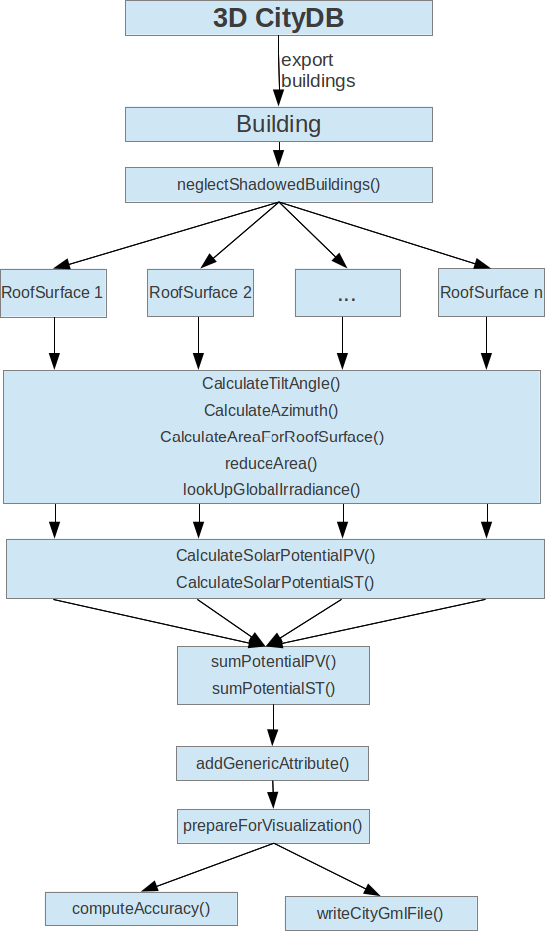
\includegraphics[width=0.5\textwidth]{phase2/group2/figure/workflow.png}
	\caption{Work flow to estimate the solar potential from 3D CityDB}
	\label{fig:workflow}
\end{figure}
\subsubsection{Related Work}\label{sec:relatedwork}
The Solar Atlas Berlin is a project which was done by the engineering office simuPLAN to estimate the solar potential of the individual building of the City of Berlin. As data source a Digital terrain Model computed from laser scanning data was used. To estimate the solar potential the roof area applicable for solar panels, tilt and azimuth of the roof surface is used. In addition also the shadowing of other buildings is considered. After developing the program and obtaining own results, the results will be compared with this data. Since, laser scanning data has been used, the equipment on the roof surface in known in detail, therefore a it is assumed from the authors that the calculated potential from Solat Atlas Berlin is from higher reliability than the potential computed from an LOD 2 MOdel, where only the roof surface is known and information about roof equipment not included. \citen{solaratlas}